\documentclass{beamer}
\usetheme{Madrid} 
\setbeamertemplate{navigation symbols}{}
\usepackage{booktabs}
\usepackage[autostyle]{csquotes}
\usepackage{multicol,lipsum,microtype}
% \usepackage[xcdraw,dvipsnames]{xcolor}
% \usepackage[backend=biber]{biblatex}
\usepackage[natbib=true,style=verbose,backend=bibtex,useprefix=true]{biblatex}
\addbibresource{presentation.tex/bib/main.bib}
\usepackage{listings}
\usepackage{lstautogobble}  % Fix relative indenting
\usepackage{xargs}
\usepackage{float}
\usepackage{tikz}
\usepackage{bytefield}
\usepackage{pgf-umlsd}
\usepackage{pgfplots}
\pgfplotsset{compat=1.16}
\usepgfplotslibrary{statistics}
\usepgfplotslibrary{groupplots}
\usepackage{caption}
\usepackage{subcaption}
\usepackage{acronym}
\usepackage{mathtools}
\usepackage{amssymb}
\usepackage{amsmath}
\usepackage{zi4}            % Nice font
\usepackage{booktabs}
\usepackage{multirow}
\usepackage{hyperref}
\usepackage[toc,page]{appendix}

\definecolor{bluekeywords}{rgb}{0.13, 0.13, 1}
\definecolor{greencomments}{rgb}{0, 0.5, 0}
\definecolor{redstrings}{rgb}{0.9, 0, 0}
\definecolor{graynumbers}{rgb}{0.5, 0.5, 0.5}

% \usetikzlibrary{external}
% \tikzexternalize[prefix=tikz/]
% \usepackage[a4paper,landscape,hmargin={1cm,1cm}]{geometry}
\usepackage{tikz-timing}[2014/10/29]
\usetikztiminglibrary[rising arrows]{clockarrows}
\usetikzlibrary{fit}
\usetikzlibrary{calc}
\usetikzlibrary{quotes}
\usetikzlibrary{positioning}
\usetikzlibrary{arrows,automata}
\usetikzlibrary{backgrounds,calc,shadings,shadows}
\usetikzlibrary{mindmap,trees}
\usetikzlibrary{patterns}
\usetikzlibrary{shapes,decorations.pathreplacing}
\let\oldfootnotesize\footnotesize
\renewcommand*{\footnotesize}{\oldfootnotesize\tiny}
\usepackage{caption}
\captionsetup[figure]{labelformat=empty}% redefines the caption setup of the figures environment in the beamer class.

\tikzstyle{bag} = [align=center]

\makeatletter
\pgfkeys{/pgf/.cd,
  parallelepiped offset x/.initial=2mm,
  parallelepiped offset y/.initial=2mm
}
\pgfdeclareshape{parallelepiped}
{
  \inheritsavedanchors[from=rectangle] % this is nearly a rectangle
  \inheritanchorborder[from=rectangle]
  \inheritanchor[from=rectangle]{north}
  \inheritanchor[from=rectangle]{north west}
  \inheritanchor[from=rectangle]{north east}
  \inheritanchor[from=rectangle]{center}
  \inheritanchor[from=rectangle]{west}
  \inheritanchor[from=rectangle]{east}
  \inheritanchor[from=rectangle]{mid}
  \inheritanchor[from=rectangle]{mid west}
  \inheritanchor[from=rectangle]{mid east}
  \inheritanchor[from=rectangle]{base}
  \inheritanchor[from=rectangle]{base west}
  \inheritanchor[from=rectangle]{base east}
  \inheritanchor[from=rectangle]{south}
  \inheritanchor[from=rectangle]{south west}
  \inheritanchor[from=rectangle]{south east}
  \backgroundpath{
    % store lower right in xa/ya and upper right in xb/yb
    \southwest \pgf@xa=\pgf@x \pgf@ya=\pgf@y
    \northeast \pgf@xb=\pgf@x \pgf@yb=\pgf@y
    \pgfmathsetlength\pgfutil@tempdima{\pgfkeysvalueof{/pgf/parallelepiped
      offset x}}
    \pgfmathsetlength\pgfutil@tempdimb{\pgfkeysvalueof{/pgf/parallelepiped
      offset y}}
    \def\ppd@offset{\pgfpoint{\pgfutil@tempdima}{\pgfutil@tempdimb}}
    \pgfpathmoveto{\pgfqpoint{\pgf@xa}{\pgf@ya}}
    \pgfpathlineto{\pgfqpoint{\pgf@xb}{\pgf@ya}}
    \pgfpathlineto{\pgfqpoint{\pgf@xb}{\pgf@yb}}
    \pgfpathlineto{\pgfqpoint{\pgf@xa}{\pgf@yb}}
    \pgfpathclose
    \pgfpathmoveto{\pgfqpoint{\pgf@xb}{\pgf@ya}}
    \pgfpathlineto{\pgfpointadd{\pgfpoint{\pgf@xb}{\pgf@ya}}{\ppd@offset}}
    \pgfpathlineto{\pgfpointadd{\pgfpoint{\pgf@xb}{\pgf@yb}}{\ppd@offset}}
    \pgfpathlineto{\pgfpointadd{\pgfpoint{\pgf@xa}{\pgf@yb}}{\ppd@offset}}
    \pgfpathlineto{\pgfqpoint{\pgf@xa}{\pgf@yb}}
    \pgfpathmoveto{\pgfqpoint{\pgf@xb}{\pgf@yb}}
    \pgfpathlineto{\pgfpointadd{\pgfpoint{\pgf@xb}{\pgf@yb}}{\ppd@offset}}
  }
}
\makeatother

\definecolor{listing-background}{HTML}{F7F7F7}
\definecolor{listing-rule}{HTML}{B3B2B3}
\definecolor{listing-numbers}{HTML}{B3B2B3}
\definecolor{listing-text-color}{HTML}{000000}
\definecolor{listing-keyword}{HTML}{435489}
\definecolor{listing-keyword-2}{HTML}{1284CA} % additional keywords
\definecolor{listing-keyword-3}{HTML}{9137CB} % additional keywords
\definecolor{listing-identifier}{HTML}{435489}
\definecolor{listing-string}{HTML}{00999A}
\definecolor{listing-comment}{HTML}{8E8E8E}

\lstset{
  language         = C++,
  numbers          = left,
  xleftmargin      = 2.7em,
  framexleftmargin = 2.5em,
  backgroundcolor  = \color{listing-background},
  basicstyle       = \color{listing-text-color}\linespread{1.0}\small\ttfamily{},
  breaklines       = true,
  frame            = single,
  framesep         = 0.19em,
  rulecolor        = \color{listing-rule},
  frameround       = ffff,
  tabsize          = 4,
  numberstyle      = \color{listing-numbers},
  aboveskip        = 1.0em,
  belowskip        = 0.1em,
  abovecaptionskip = 0em,
  belowcaptionskip = 1.0em,
  keywordstyle     = {\color{listing-keyword}\bfseries},
  keywordstyle     = {[2]\color{listing-keyword-2}\bfseries},
  keywordstyle     = {[3]\color{listing-keyword-3}\bfseries\itshape},
  sensitive        = true,
  identifierstyle  = \color{listing-identifier},
  commentstyle     = \color{listing-comment},
  stringstyle      = \color{listing-string},
  showstringspaces = false,
  escapeinside     = {/*@}{@*/}, % Allow LaTeX inside these special comments
  literate         =
  {á}{{\'a}}1 {é}{{\'e}}1 {í}{{\'i}}1 {ó}{{\'o}}1 {ú}{{\'u}}1
  {Á}{{\'A}}1 {É}{{\'E}}1 {Í}{{\'I}}1 {Ó}{{\'O}}1 {Ú}{{\'U}}1
  {à}{{\`a}}1 {è}{{\'e}}1 {ì}{{\`i}}1 {ò}{{\`o}}1 {ù}{{\`u}}1
  {À}{{\`A}}1 {È}{{\'E}}1 {Ì}{{\`I}}1 {Ò}{{\`O}}1 {Ù}{{\`U}}1
  {ä}{{\"a}}1 {ë}{{\"e}}1 {ï}{{\"i}}1 {ö}{{\"o}}1 {ü}{{\"u}}1
  {Ä}{{\"A}}1 {Ë}{{\"E}}1 {Ï}{{\"I}}1 {Ö}{{\"O}}1 {Ü}{{\"U}}1
  {â}{{\^a}}1 {ê}{{\^e}}1 {î}{{\^i}}1 {ô}{{\^o}}1 {û}{{\^u}}1
  {Â}{{\^A}}1 {Ê}{{\^E}}1 {Î}{{\^I}}1 {Ô}{{\^O}}1 {Û}{{\^U}}1
  {œ}{{\oe}}1 {Œ}{{\OE}}1 {æ}{{\ae}}1 {Æ}{{\AE}}1 {ß}{{\ss}}1
  {ç}{{\c c}}1 {Ç}{{\c C}}1 {ø}{{\o}}1 {å}{{\r a}}1 {Å}{{\r A}}1
  {€}{{\EUR}}1 {£}{{\pounds}}1 {«}{{\guillemotleft}}1
  {»}{{\guillemotright}}1 {ñ}{{\~n}}1 {Ñ}{{\~N}}1 {¿}{{?`}}1
  {…}{{\ldots}}1 {≥}{{>=}}1 {≤}{{<=}}1 {„}{{\glqq}}1 {“}{{\grqq}}1
  {”}{{''}}1
}
\lstdefinelanguage{none}{
  identifierstyle=,
  commentstyle=,
  stringstyle=,
  keywordstyle=,
}

\def\lav{lavander!90}
\def\oran{orange!30}

\AtBeginSection[]
{
  \begin{frame}
    \frametitle{Table of Contents}
    \tableofcontents[currentsection]
  \end{frame}
}

\title{LoRa une approche bottom-up}
\subtitle{}
\author{Thomas Perale}

\date{Smartmonday Decembre 2020}

\begin{document}
\frame{\maketitle}

\begin{frame}{Table of Content}
    % We are going to start at a very high level overview to then dig into the
    % more detailled aspect of LoRa.
    \tableofcontents
\end{frame}

\section{Introduction}

\subsection{Introduction}

\begin{frame}{Introduction}
\framesubtitle{Internet of Things}
\begin{center}
\makebox[\linewidth]{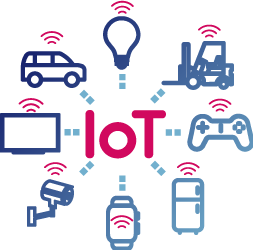
\includegraphics[page=1,width=0.3\paperwidth]{presentation.tex/fig/iot.png}}
\end{center}
\end{frame}

\subsection{LPWAN}

\begin{frame}{Introduction}
\framesubtitle{LPWAN}
\begin{center}
\scalebox{0.6}{%
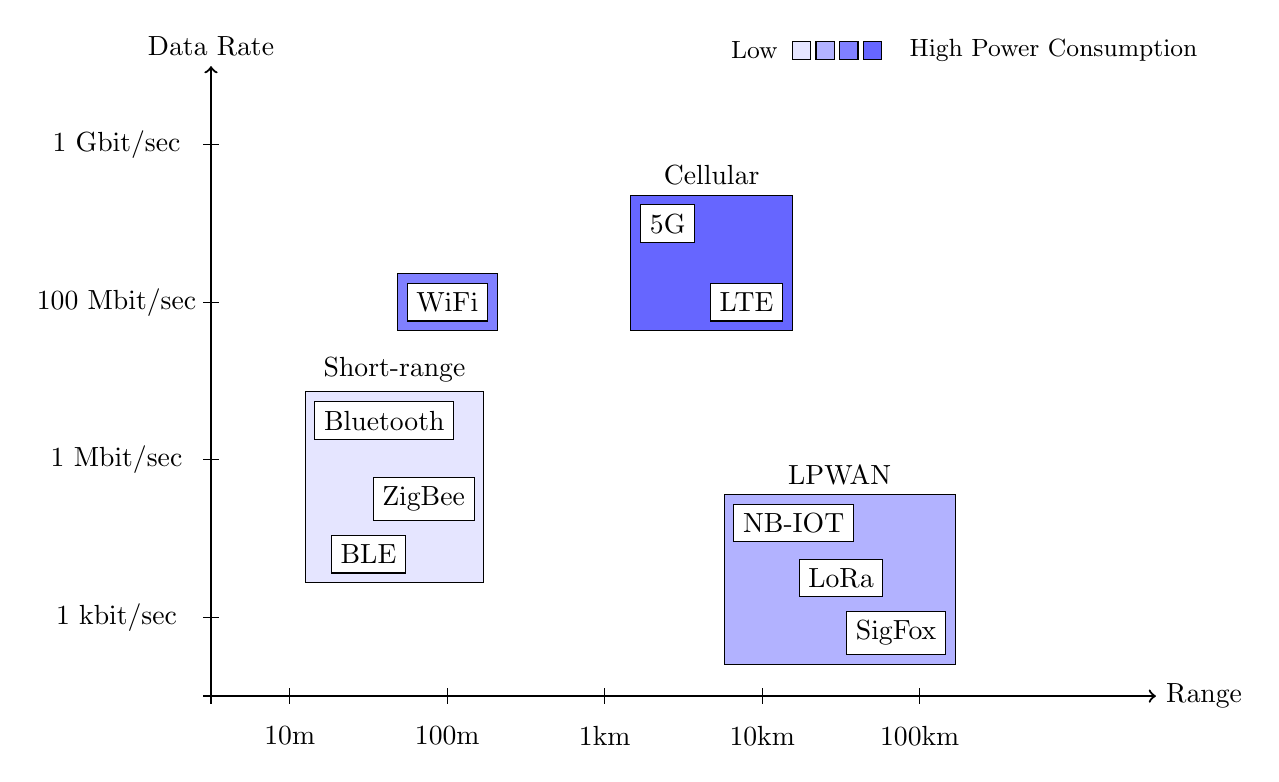
\begin{tikzpicture}
  \draw[->,thick] (-0.1,0)--(12,0) node[right]{Range};
  \draw[->,thick] (0,-0.1)--(0,8) node[above]{Data Rate};
  \node[] at (1, -0.5) {10m};
  \draw[] (1,-0.1)--(1,0.1);
  \node[] at (3, -0.5) {100m};
  \draw[] (3,-0.1)--(3,0.1);
  \node[] at (5, -0.5) {1km};
  \draw[] (5,-0.1)--(5,0.1);
  \node[] at (7, -0.5) {10km};
  \draw[] (7,-0.1)--(7,0.1);
  \node[] at (9, -0.5) {100km};
  \draw[] (9,-0.1)--(9,0.1);

  \node[] at (-1.2, 1) {1 kbit/sec};
  \draw[] (-0.1,1)--(0.1,1);
  \node[] at (-1.2, 3) {1 Mbit/sec};
  \draw[] (-0.1,3)--(0.1,3);
  \node[] at (-1.2, 5) {100 Mbit/sec};
  \draw[] (-0.1,5)--(0.1,5);
  \node[] at (-1.2, 7) {1 Gbit/sec};
  \draw[] (-0.1,7)--(0.1,7);

  \node[draw,fill=white] at (8,1.5) (lora) {LoRa};
  \node[draw,fill=white] at (8.7,0.8) (sigfox) {SigFox};
  \node[draw,fill=white] at (7.4,2.2) (nb) {NB-IOT};
  \begin{scope}[on background layer]
    \node[draw,fill=blue!30,fit=(lora) (sigfox) (nb), label=above:{LPWAN}] {};
  \end{scope}

  \node[draw,fill=white] at (2.2,3.5) (bluetooth) {Bluetooth};
  \node[draw,fill=white] at (2.7,2.5) (zigbee) {ZigBee};
  \node[draw,fill=white] at (2.0,1.8) (ble) {BLE};
  \begin{scope}[on background layer]
    \node[draw,fill=blue!10,fit=(bluetooth) (zigbee) (ble), label=above:{Short-range}] {};
  \end{scope}

  \node[draw,fill=white] at (3,5) (wifi) {WiFi};
  \begin{scope}[on background layer]
    \node[draw,fill=blue!50,fit=(wifi)] {};
  \end{scope}

  \node[draw,fill=white] at (6.8,5) (lte) {LTE};
  \node[draw,fill=white] at (5.8,6) (5g) {5G};
  \begin{scope}[on background layer]
    \node[draw,fill=blue!60,fit=(lte) (5g), label=above:{Cellular}] {};
  \end{scope}

  \node[] at (6.9,8.2) (leg5) {\small Low};
  \node[draw,fill=blue!10] at (7.5,8.2) (leg1) {};
  \node[draw,fill=blue!30] at (7.8,8.2) (leg2) {};
  \node[draw,fill=blue!50] at (8.1,8.2) (leg3) {};
  \node[draw,fill=blue!60] at (8.4,8.2) (leg4) {};
  \node[] at (10.7,8.2) (leg5) {\small High Power Consumption};
\end{tikzpicture}
}
\end{center}

\end{frame}

\begin{frame}{Introduction}
\framesubtitle{LPWAN}
\begin{columns}
  \begin{column}{0.5\textwidth}
  \begin{itemize}
    \item Longue portée (7-15km)
    \item Faible débit
    \begin{itemize}
      \item $<$ kb/sec
      \item Dizaine de messages par jours
    \end{itemize}
    \item Basse consommation
    \begin{itemize}
      \item Plusieurs années de batterie
    \end{itemize}
    \item Prix faible
    \begin{itemize}
      \item Module à 2.5€
    \end{itemize}
    \item Topologie en étoile
  \end{itemize}
  \end{column}
  \begin{column}{0.5\textwidth}
  \begin{center}
\scalebox{0.6}{
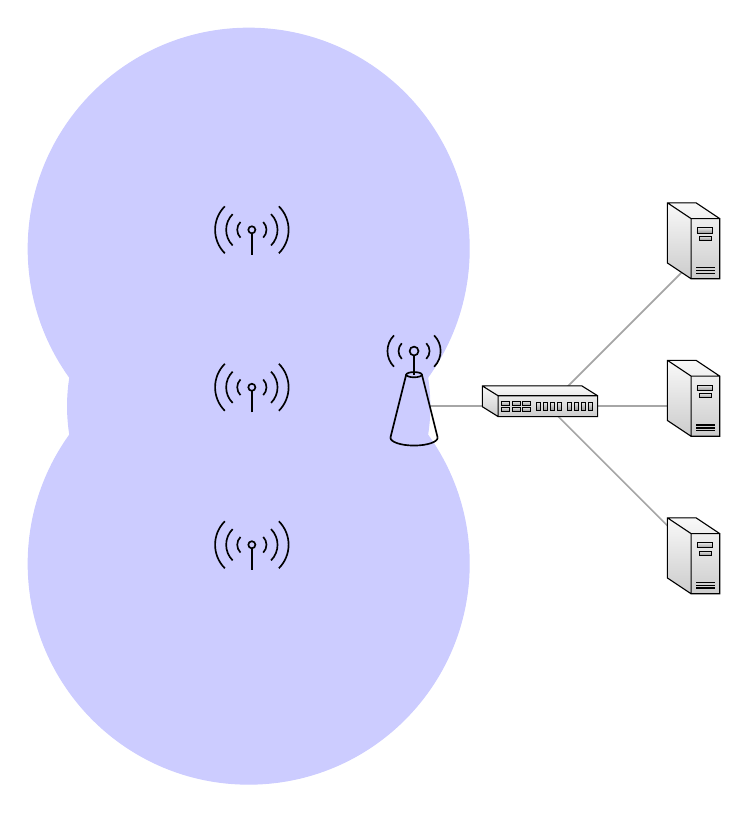
\begin{tikzpicture}[
  radiation/.style={{decorate,decoration={expanding waves,angle=90,segment length=4pt}}},
  ports/.style={
    line width=0.3pt,
    top color=gray!20,
    bottom color=gray!80
  },
  rack switch/.style={
    minimum width=1.25cm,
    minimum height=0.25cm,
    parallelepiped,fill=white, draw,
    parallelepiped offset x=2mm,
    parallelepiped offset y=1.25mm,
    xscale=-1,
    path picture={
      \draw[top color=gray!5,bottom color=gray!40]
      (path picture bounding box.south west) rectangle
      (path picture bounding box.north east);
      \coordinate (A-west) at ([xshift=-0.2cm]path picture bounding box.west);
      \coordinate (A-center) at ($(path picture bounding box.center)!0!(path
        picture bounding box.south)$);
      \foreach \x in {0.275,0.525,0.775}{
        \draw[ports]([yshift=-0.05cm]$(A-west)!\x!(A-center)$)
          rectangle +(0.1,0.05);
        \draw[ports]([yshift=-0.125cm]$(A-west)!\x!(A-center)$)
          rectangle +(0.1,0.05);
       }
      \coordinate (A-east) at (path picture bounding box.east);
      \foreach \x in {0.085,0.21,0.335,0.455,0.635,0.755,0.875,1}{
        \draw[ports]([yshift=-0.1125cm]$(A-east)!\x!(A-center)$)
          rectangle +(0.05,0.1);
      }
    }
  },
  server/.style={
    fill=white, draw,
    minimum width=0.35cm,
    minimum height=0.75cm,
    parallelepiped,
    parallelepiped offset x=3mm,
    parallelepiped offset y=2mm,
    xscale=-1,
    path picture={
      \draw[top color=gray!5,bottom color=gray!40]
      (path picture bounding box.south west) rectangle
      (path picture bounding box.north east);
      \coordinate (A-center) at ($(path picture bounding box.center)!0!(path
        picture bounding box.south)$);
      \coordinate (A-west) at ([xshift=-0.575cm]path picture bounding box.west);
      \draw[ports]([yshift=0.1cm]$(A-west)!0!(A-center)$)
        rectangle +(0.2,0.065);
      \draw[ports]([yshift=0.01cm]$(A-west)!0.085!(A-center)$)
        rectangle +(0.15,0.05);
      \fill[black]([yshift=-0.35cm]$(A-west)!-0.1!(A-center)$)
        rectangle +(0.235,0.0175);
      \fill[black]([yshift=-0.385cm]$(A-west)!-0.1!(A-center)$)
        rectangle +(0.235,0.0175);
      \fill[black]([yshift=-0.42cm]$(A-west)!-0.1!(A-center)$)
        rectangle +(0.235,0.0175);
    }
  },
  antenna/.pic={
    code={\tikzset{scale=2/10}
      \draw[semithick] (0,0) -- (1,4);% left line
      \draw[semithick] (3,0) -- (2,4);% right line
      \draw[semithick] (0,0) arc (180:0:1.5 and -0.5);
      \node[inner sep=4pt] (circ) at (1.5,5.5) {};
      \draw[semithick] (1.5,5.5) circle(8pt);
      \draw[semithick] (1.5,5.5cm-8pt) -- (1.5,4);
      \draw[semithick] (1.5,4) ellipse (0.5 and 0.166);
      \draw[semithick,radiation,decoration={angle=45}] (1.5cm+8pt,5.5) -- +(0:2);
      \draw[semithick,radiation,decoration={angle=45}] (1.5cm-8pt,5.5) -- +(180:2);
    }
  },
  node/.pic={
    code={\tikzset{scale=2/10}
      \draw[semithick] (1.5,-0.5) -- (1.5,1.5cm-8pt);
      \draw[semithick] (1.5,1.5) circle(8pt);
      \draw[semithick,radiation,decoration={angle=45}] (1.5cm+8pt,1.5) -- +(0:3);
      \draw[semithick,radiation,decoration={angle=45}] (1.5cm-8pt,1.5) -- +(180:3);
    }
  }
]
  \draw[color=blue!20,fill=blue!20] (-1.8,2) circle (2.8cm);
  \draw[color=blue!20,fill=blue!20] (-1.8,0) circle (2.3cm);
  \draw[color=blue!20,fill=blue!20] (-1.8,-2) circle (2.8cm);

  \path (0.5,0) edge [-,semithick,draw=gray!70] (2,0);
  \path (2,0) edge [-,semithick,draw=gray!70] (4,2);
  \path (2,0) edge [-,semithick,draw=gray!70] (4,0);
  \path (2,0) edge [-,semithick,draw=gray!70] (4,-2);

  \path (0,-0.4) pic [fill=white,scale=1] {antenna};

  \path (-2,2) pic [black,scale=0.8] {node};
  \path (-2,0) pic [black,scale=0.8] {node};
  \path (-2,-2) pic [black,scale=0.8] {node};

  \node[rack switch] at (2,0) {};

  \node[server] (loraserv) at (4,0) {};
  \node[server] (loraserv) at (4,2) {};
  \node[server] (loraserv) at (4,-2) {};
\end{tikzpicture}
}
\end{center}
 
    
  \end{column}
\end{columns}
\end{frame}

\subsection{Network Stack}

\begin{frame}{Introduction}
\framesubtitle{Network Stack}
\begin{center}
\scalebox{0.8}{%
\begin{tikzpicture}[auto,node distance=1.2cm]
  \tikzstyle{comment}=[ right=2pt, font=\small, fill=white, text=black, draw=black, ]
  \tikzstyle{every state}=[rectangle,thick,draw=black,fill=gray!20,text=black, minimum width= 6cm, minimum height= 1.00cm ]
  \tikzstyle{smallstate}=[rectangle,thick,draw=black!80,fill=gray!10,text=black, minimum width= 6cm, minimum height= 0.25cm ]
  \tikzstyle{innerstate}=[rectangle,thick,draw=black,fill=gray!10,text=black, minimum width= 4cm, minimum height= 1.00cm ]

  \only<1>{
    \node[state] at (0, 0) (A)                  {Application Layer};
    \node[state]         (B) [below of=A]       {Presentation Layer};
    \node[state]         (C) [below of=B]       {Session Layer};
    \node[state]         (D) [below of=C]       {Transport Layer};
    \node[state]         (E) [below of=D]       {Network Layer};
    \node[state]         (F) [below of=E]       {Data Link Layer (MAC+LLC)};
    \node[state]         (G) [below of=F]       {Physical Layer};
    \draw[decorate,decoration={brace,amplitude=8pt},xshift=-5pt,yshift=0pt,black!50] (D.south west) -- (B.north west) node[black!50,midway,left,xshift=-26pt] {\tiny Abstraction};
  }

  \only<2>{
    \node[state] at (0, 0) (A)                  {Application Layer};
    \node[smallstate]    (B) [below of=A]       {...};
    \node[state]         (E) [below of=B]       {Network Layer};
    \node[state]         (F) [below of=E]       {Data Link Layer (MAC+LLC)};
    \node[state]         (G) [below of=F]       {Physical Layer};
    \draw[decorate,decoration={brace,amplitude=8pt},xshift=-5pt,yshift=0pt,white] (D.south west) -- (B.north west) node[white,midway,left,xshift=-26pt] {\tiny Abstraction};

    \draw[decorate,decoration={brace,amplitude=8pt},xshift=-5pt,yshift=0pt,black!70] (E.south west) -- (E.north west) node[black!70,midway,left,xshift=-6pt] {\tiny Internet Integration};
    \draw[decorate,decoration={brace,amplitude=8pt},xshift=-5pt,yshift=0pt,black!70] (F.south west) -- (F.north west) node[black!70,midway,left,xshift=-6pt] {\tiny Access};
    \draw[decorate,decoration={brace,amplitude=8pt},xshift=-5pt,yshift=0pt,black!70] (G.south west) -- (G.north west) node[black!70,midway,left,xshift=-6pt] {\tiny Radio Comm};
  }

\end{tikzpicture}
}
\end{center}

\end{frame}

\begin{frame}{Introduction}
\framesubtitle{Network Stack}
\begin{center}
\scalebox{0.8}{%
\begin{tikzpicture}[auto,node distance=1.2cm]
  \tikzstyle{comment}=[ right=2pt, font=\small, fill=white, text=black, draw=black, ]
  \tikzstyle{every state}=[rectangle,thick,draw=black,fill=gray!20,text=black, minimum width= 6cm, minimum height= 1.00cm ]
  \tikzstyle{smallstate}=[rectangle,thick,draw=black!80,fill=gray!10,text=black, minimum width= 6cm, minimum height= 0.25cm ]
  \tikzstyle{innerstate}=[rectangle,thick,draw=black,fill=gray!10,text=black, minimum width= 4cm, minimum height= 1.00cm ]

  \node[state] at (0, 0) (A)                  {Application};
  \node[smallstate]    (B) [below of=A]       {...};
  \node[state]         (E) [below of=B]       {Network};
  \node[state]         (F) [below of=E]       {Data Link};
  \node[state]         (G) [below of=F]       {Physical};
  \draw[decorate,decoration={brace,amplitude=8pt},xshift=-5pt,yshift=0pt,white] (D.south west) -- (B.north west) node[white,midway,left,xshift=-26pt] {\tiny Abstraction};

  \draw[decorate,decoration={brace,amplitude=8pt},xshift=-5pt,yshift=0pt,black!70] (E.south west) -- (E.north west) node[black!70,midway,left,xshift=-6pt] {\tiny Internet Integration};
  \draw[decorate,decoration={brace,amplitude=8pt},xshift=-5pt,yshift=0pt,black!70] (F.south west) -- (F.north west) node[black!70,midway,left,xshift=-6pt] {\tiny Access};
  \draw[decorate,decoration={brace,amplitude=8pt},xshift=-5pt,yshift=0pt,black!70] (G.south west) -- (G.north west) node[black!70,midway,left,xshift=-6pt] {\tiny Radio Comm};
\end{tikzpicture}
}
\end{center}

\end{frame}


\section{LoRa}

\subsection{Introduction}

\begin{frame}{LoRa}
\framesubtitle{Introduction}
\begin{center}
\scalebox{0.8}{%
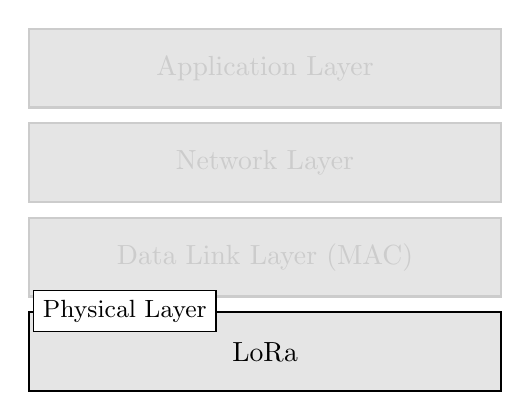
\begin{tikzpicture}[auto,node distance=1.2cm]
  \tikzstyle{comment}=[ right=2pt, font=\small, fill=white, text=black, draw=black, ]
  \tikzstyle{every state}=[rectangle,thick,draw=black,fill=gray!20,text=black, minimum width= 6cm, minimum height= 1.00cm ]
  \tikzstyle{smallstate}=[rectangle,thick,draw=black!80,fill=gray!10,text=black, minimum width= 6cm, minimum height= 0.25cm ]
  \tikzstyle{innerstate}=[rectangle,thick,draw=black,fill=gray!10,text=black, minimum width= 4cm, minimum height= 1.00cm ]

  \node[state,color=gray!40,fill=gray!20] at (0, 0) (A)            { Application Layer };
  \node[state,color=gray!40,fill=gray!20]         (E) [below of=A] { Network Layer };
  \node[state,color=gray!40,fill=gray!20]         (F) [below of=E] { Data Link Layer (MAC) };
  \node[state]         (G) [below of=F]                            { LoRa };

  \node[comment]       at (G.north west) {Physical Layer};
\end{tikzpicture}
}
\end{center}

\end{frame}

\begin{frame}{LoRa}
\framesubtitle{Radio Frequence}
\makebox[\linewidth]{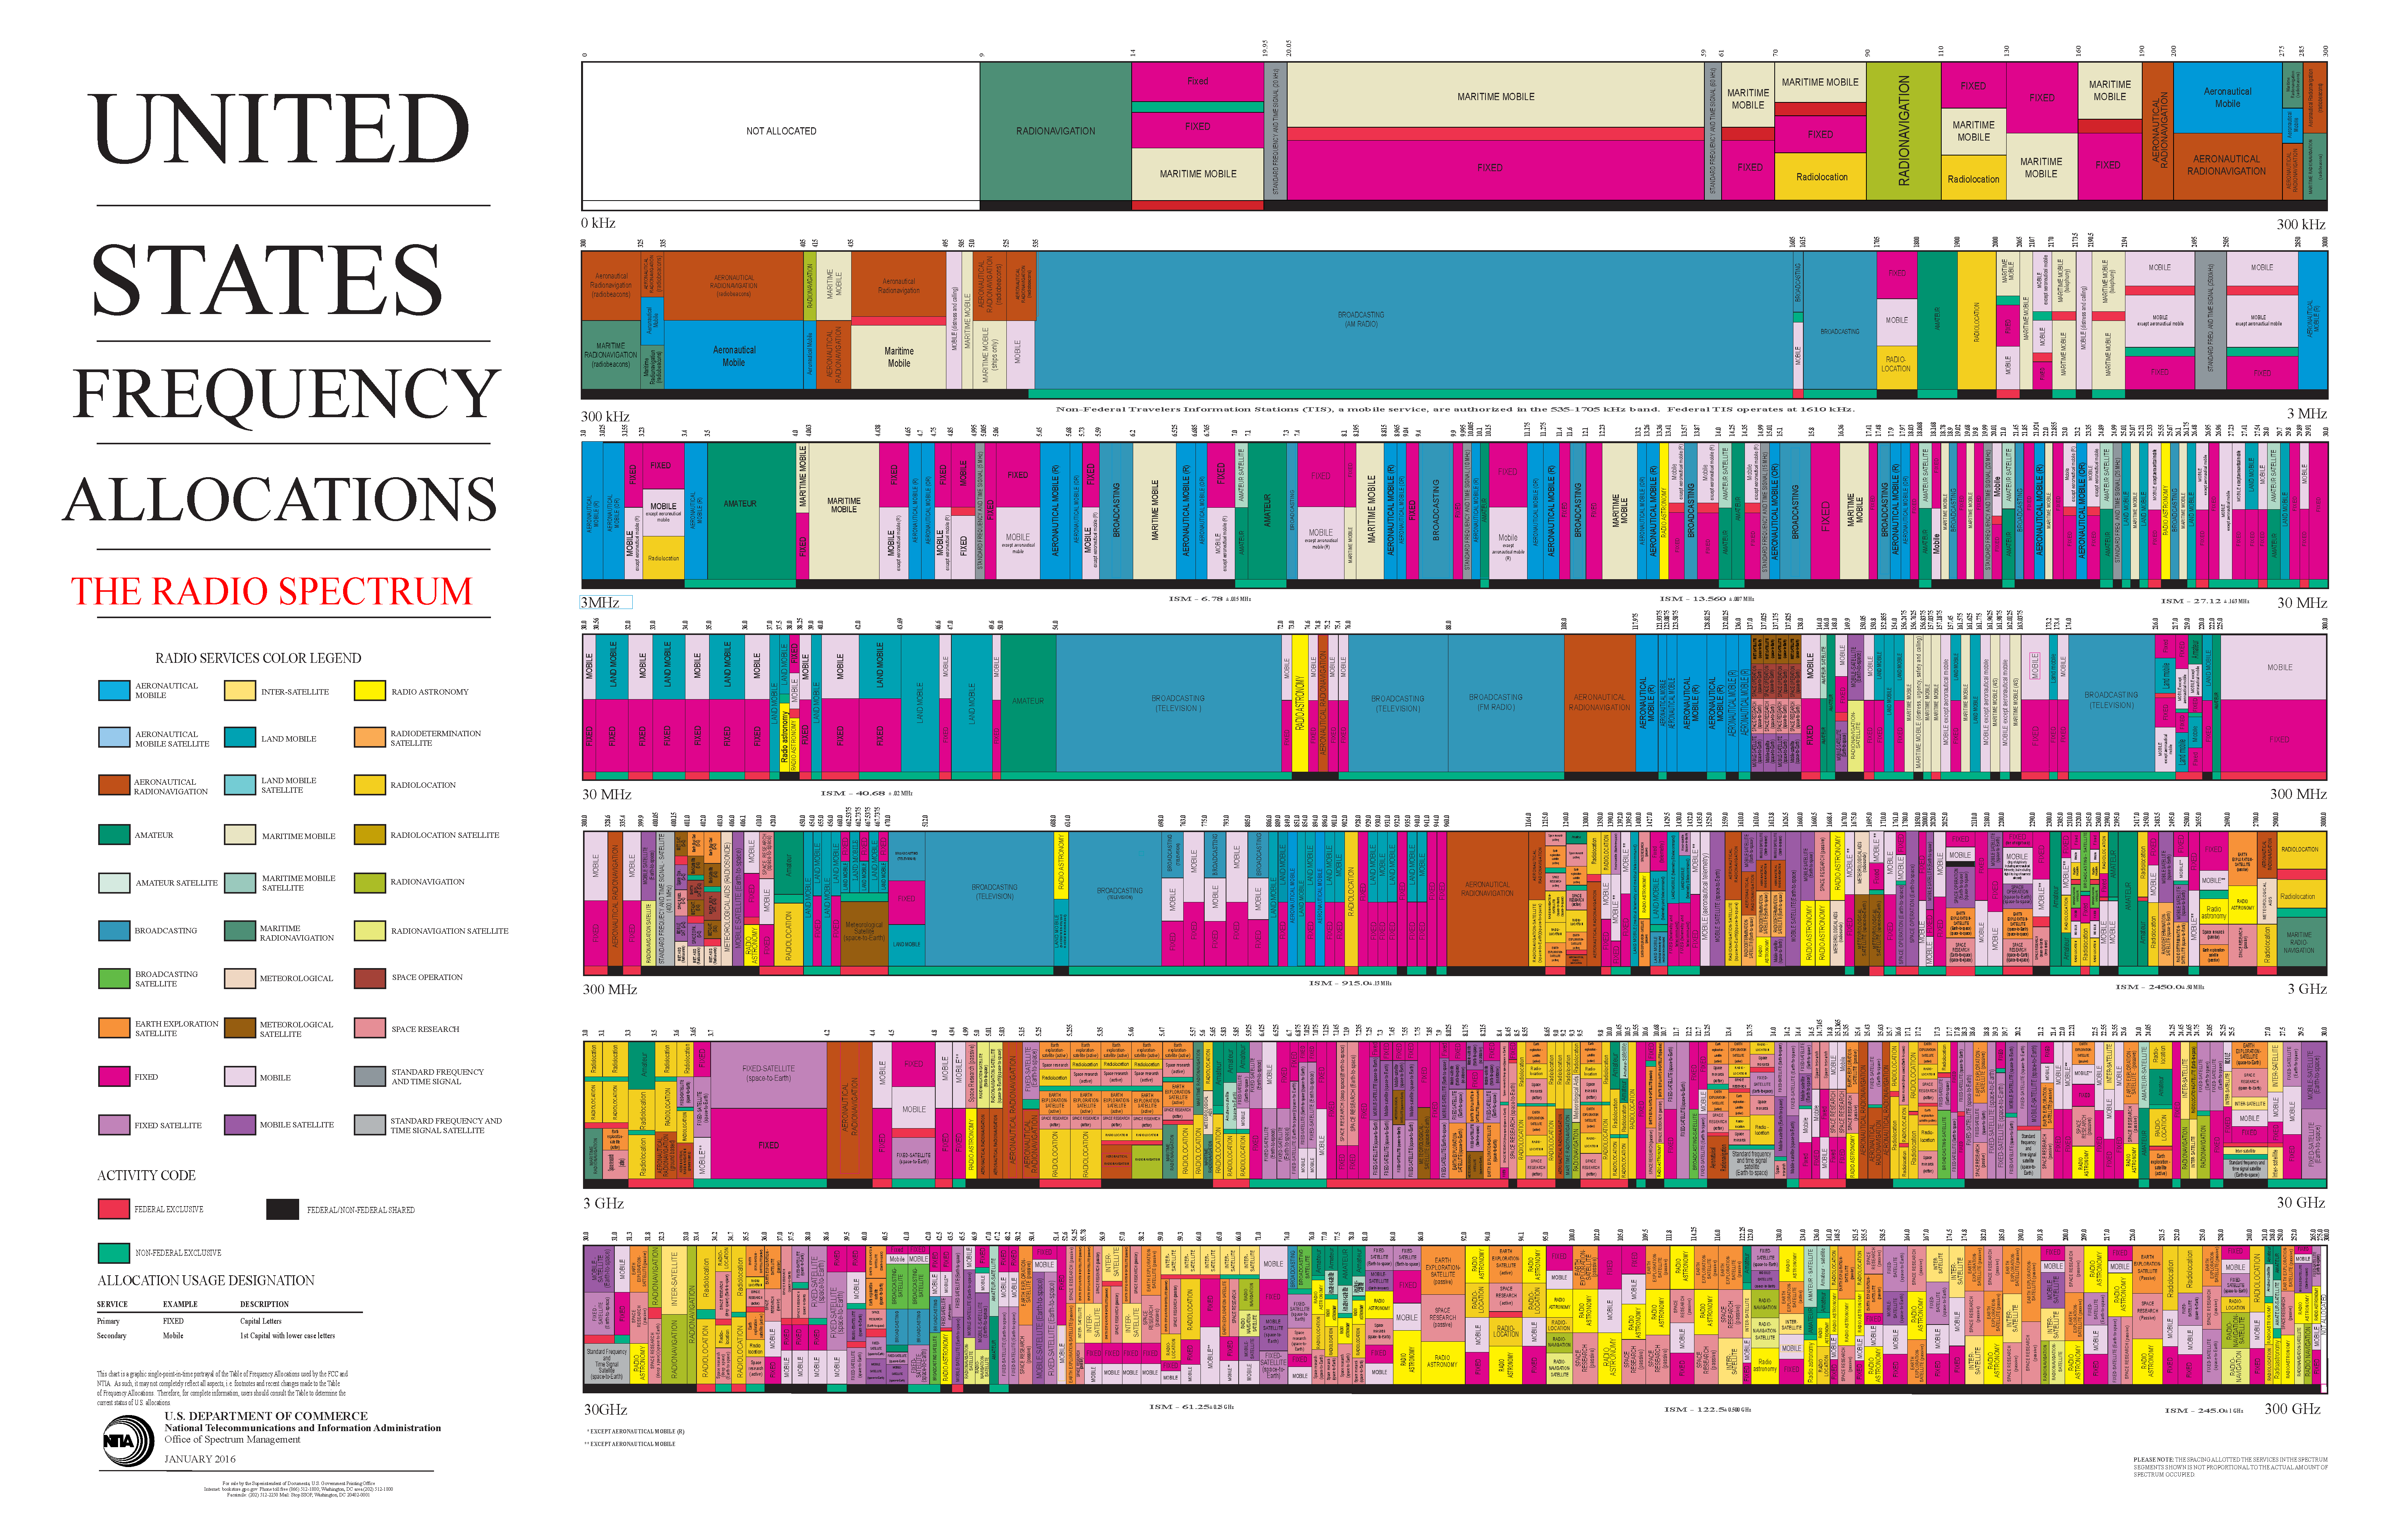
\includegraphics[page=1,width=\paperwidth]{presentation.tex/fig/frequencychart.pdf}}
\end{frame}

\begin{frame}{LoRa}
\framesubtitle{Modulation}
\begin{block}{}
{
Comment transmettre de l'information en utilisant une radio ?
}
\end{block}

\end{frame}


\begin{frame}{LoRa}
\framesubtitle{Modulation}
\begin{columns}
\begin{column}{0.5\textwidth}
\begin{itemize}
  \item Signal Analogique
  \begin{itemize}
    \item Voix
    \item Musique
    \item Walkie-talkie
    \item ...
  \end{itemize}
  \item Modulation Analogique
  \begin{itemize}
    \only<1->{\item Modulation de l'amplitude}
    \only<2->{\item Modulation de la frequence}
  \end{itemize}
\end{itemize}  
\end{column}
\begin{column}{0.5\textwidth}
\begin{center}
\scalebox{0.6}{%
\begin{tikzpicture}[samples=1000, domain=0:10*pi]
\begin{axis}[
  width=11cm, height=3.5cm,
  xtick=\empty,
  ytick=\empty,
  xlabel={\large $t$},
  ylabel={\large $x(t)$},
  xmin=0, xmax=11,
  ymin=-3, ymax=5,
  axis lines = middle,
  very thick,
  trig format = rad
]
  \addplot [no markers, smooth, thick] {2.5 + 2*sin(2*pi*0.25*x)};
\end{axis}
  
\begin{axis}[
  at={(0, -2.25cm)},
  width=11cm, height=3.5cm,
  xtick=\empty,
  ytick=\empty,
  xlabel={\large $t$},
  ylabel={\textcolor{blue!60}{carrier wave}},
  xmin=0, xmax=11,
  ymin=-3, ymax=5,
  axis lines = middle,
  very thick,
  trig format = rad
]
  \addplot [no markers, smooth, blue!60, very thick] {2*sin(6*pi*x)};
\end{axis}
  
\only<1>{
\begin{axis}[
  at={(0, -4.5cm)},
  width=11cm, height=3.5cm,
  xtick=\empty,
  ytick=\empty,
  xlabel={\large $t$},
  ylabel={\textcolor{red!60}{AM wave}},
  xmin=0, xmax=11,
  ymin=-3, ymax=5,
  axis lines = middle,
  very thick,
  trig format = rad
]
\addplot expression [no markers, smooth, red!60, very thick] {(2.5 + sin(0.5*pi*x)) * sin(6*pi*x)};
\end{axis}
}

\only<2>{
\begin{axis}[
  at={(0, -4.5cm)},
  width=11cm, height=3.5cm,
  xtick=\empty,
  ytick=\empty,
  xlabel={\large $t$},
  ylabel={\textcolor{green!30!black}{FM wave}},
  xmin=0, xmax=11,
  ymin=-3, ymax=5,
  axis lines = middle,
  very thick,
  trig format = rad
]
  \addplot expression [no markers, smooth, green!30!black, very thick] {2*sin(2*pi*3*x - 8*cos(2*pi*0.25*x))};
\end{axis}
}
\end{tikzpicture}
}
\end{center}

\end{column}
\end{columns}


\end{frame}

\begin{frame}{LoRa}
\framesubtitle{Modulation Digitale}

\begin{block}{}
{
Comment transmettre de l'information numerique avec une radio ?
}
\end{block}

\end{frame}

\begin{frame}{LoRa}
\framesubtitle{Modulation Digitale}

\begin{columns}
\begin{column}{0.5\textwidth}
\begin{itemize}
  \item
\end{itemize}  
\end{column}
\begin{column}{0.5\textwidth}
  
\end{column}
\end{columns}
\end{frame}

\begin{frame}{LoRa}
\framesubtitle{Qu'est-ce que LoRa ?}
\begin{columns}
  \begin{column}{0.6\textwidth}
    
  \begin{itemize}
    \item Une methode de modulation propriétaire
    \begin{itemize}
      \item Creer par Semtech
      \item Grenoble, France
    \end{itemize}
    \item Transmet sur la bande ISM
    \begin{itemize}
      \item 868MHz
    \end{itemize}
    \item Longue distance de transmission
    \item Basse consommation
  \end{itemize}
  \end{column}
  \begin{column}{0.4\textwidth}
    \makebox[\linewidth]{
\includegraphics[page=1,width=0.5\paperwidth]{presentation.tex/fig/lora.png}}
  \end{column}
\end{columns}
\end{frame}

\begin{frame}{LoRa}
\framesubtitle{Chirp Spread Spectrum}
\begin{columns}
  \begin{column}{0.5\textwidth}
    \begin{center}
\scalebox{0.8}{
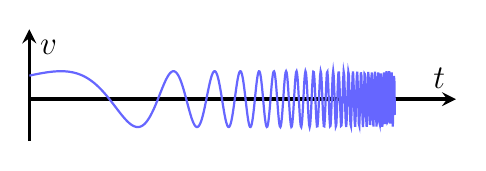
\begin{tikzpicture}
\begin{axis}[
  samples=700,
  domain=0:3*pi,
  width=7cm, height=3cm,
  xtick=\empty,
  ytick=\empty,
  xlabel={\large $t$},
  ylabel={\large $v$},
  xmin=0, xmax=11,
  ymin=-3, ymax=5,
  axis lines = middle,
  very thick,
  trig format = rad
]
\addplot[thick, blue!60]plot (\x, {2*sin(pow(2,(0.8*\x)))});
\end{axis}
\end{tikzpicture}
}
\end{center}

  \end{column}
  \begin{column}{0.5\textwidth}
    \begin{center}
      \makebox[\linewidth]{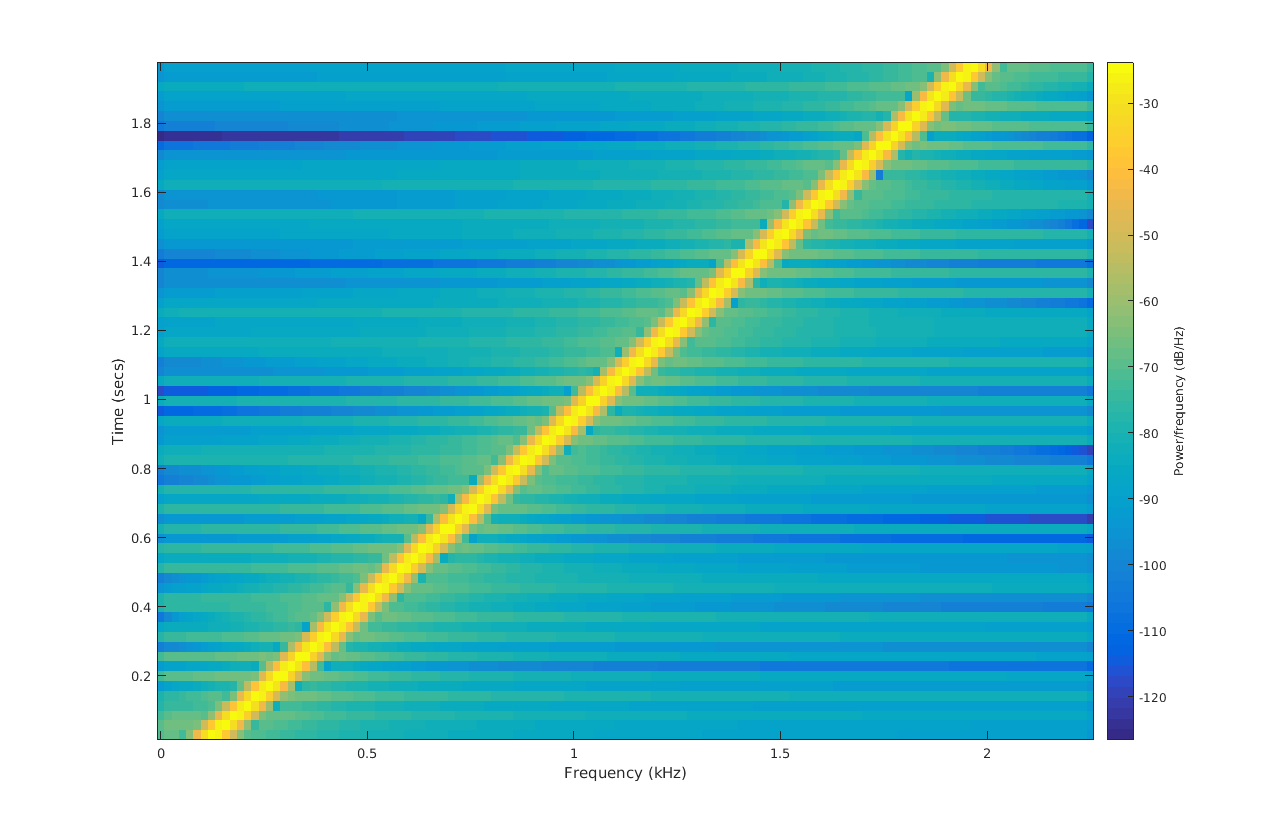
\includegraphics[page=1,width=0.55\paperwidth]{presentation.tex/fig/upchirp.png}}
    \end{center}
  \end{column}
\end{columns}

\end{frame}

\begin{frame}{LoRa}
\framesubtitle{Bandwidth}
\end{frame}

\begin{frame}{LoRa}
\framesubtitle{Channels}
\end{frame}

\begin{frame}{LoRa}
\framesubtitle{Spreading Factor}
\begin{center}
\scalebox{0.6}{%
\begin{tikzpicture}[
  arr/.style={help lines,black!70,<->},
]
  \draw[thick,-latex] (0,-2) -- (0,2)node[left] {frequency};
  \draw[thick,-latex] (-1,0) -- (11.5,0)node[below] {time};
  \draw[dashed] (1.5,-2) -- (1.5,2);
  \draw[dashed] (4.5,-2) -- (4.5,2);
  \draw[dashed] (10.5,-2) -- (10.5,2);
  \draw[] (0,-1.8) -- (1.5,1.8);
  \draw[] (1.5,-1.8) -- (4.5,1.8);
  \draw[] (4.5,-1.8) -- (10.5,1.8);

  \draw[arr] (0.1, -2.2) -- node[fill=white] {$SF7$} (1.4, -2.2);
  \draw[arr] (1.6, -2.2) -- node[fill=white] {$SF8$} (4.4, -2.2);
  \draw[arr] (4.6, -2.2) -- node[fill=white] {$SF9$} (10.4, -2.2);
\end{tikzpicture}
}
\end{center}

\end{frame}


\section{LoRaWAN}

\subsection{Introduction}

\begin{frame}{LoRaWAN}
\framesubtitle{Introduction}
\begin{center}
\scalebox{0.8}{%
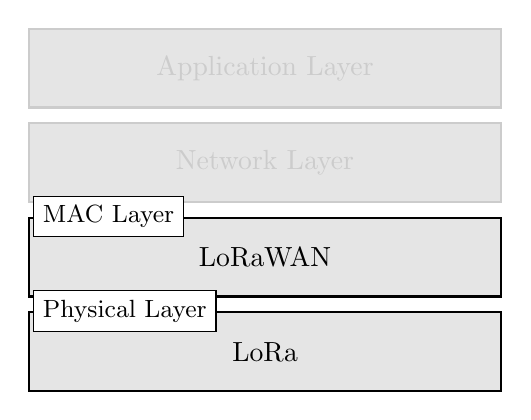
\begin{tikzpicture}[auto,node distance=1.2cm]
  \tikzstyle{comment}=[ right=2pt, font=\small, fill=white, text=black, draw=black, ]
  \tikzstyle{every state}=[rectangle,thick,draw=black,fill=gray!20,text=black, minimum width= 6cm, minimum height= 1.00cm ]
  \tikzstyle{smallstate}=[rectangle,thick,draw=black!80,fill=gray!10,text=black, minimum width= 6cm, minimum height= 0.25cm ]
  \tikzstyle{innerstate}=[rectangle,thick,draw=black,fill=gray!10,text=black, minimum width= 4cm, minimum height= 1.00cm ]

  \node[state,color=gray!40,fill=gray!20] at (0, 0) (A)            { Application Layer};
  \node[state,color=gray!40,fill=gray!20]         (E) [below of=A] { Network Layer};
  \node[state]         (F) [below of=E]                            { LoRaWAN };
  \node[state]         (G) [below of=F]                            { LoRa };

  \node[comment]       at (F.north west) {MAC Layer};
  \node[comment]       at (G.north west) {Physical Layer};
\end{tikzpicture}
}
\end{center}

\end{frame}

\subsection{LoRaWAN ?}

\begin{frame}{LoRaWAN}
\framesubtitle{Organisation de LoRaWAN}
% Photo gateway + schema organisation
\begin{columns}
  \begin{column}{0.5\textwidth}
    \begin{center}
\scalebox{0.6}{
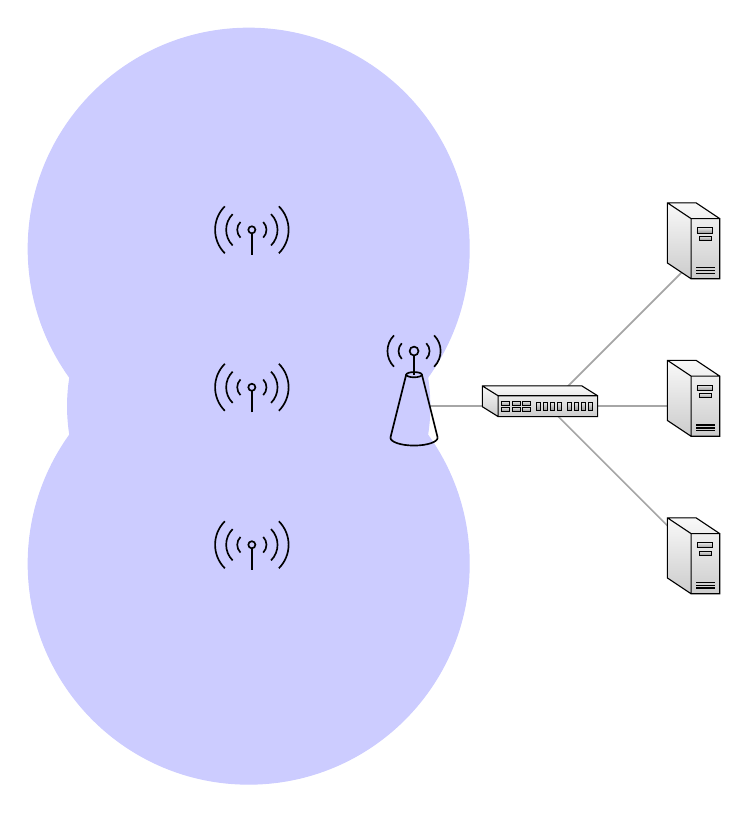
\begin{tikzpicture}[
  radiation/.style={{decorate,decoration={expanding waves,angle=90,segment length=4pt}}},
  ports/.style={
    line width=0.3pt,
    top color=gray!20,
    bottom color=gray!80
  },
  rack switch/.style={
    minimum width=1.25cm,
    minimum height=0.25cm,
    parallelepiped,fill=white, draw,
    parallelepiped offset x=2mm,
    parallelepiped offset y=1.25mm,
    xscale=-1,
    path picture={
      \draw[top color=gray!5,bottom color=gray!40]
      (path picture bounding box.south west) rectangle
      (path picture bounding box.north east);
      \coordinate (A-west) at ([xshift=-0.2cm]path picture bounding box.west);
      \coordinate (A-center) at ($(path picture bounding box.center)!0!(path
        picture bounding box.south)$);
      \foreach \x in {0.275,0.525,0.775}{
        \draw[ports]([yshift=-0.05cm]$(A-west)!\x!(A-center)$)
          rectangle +(0.1,0.05);
        \draw[ports]([yshift=-0.125cm]$(A-west)!\x!(A-center)$)
          rectangle +(0.1,0.05);
       }
      \coordinate (A-east) at (path picture bounding box.east);
      \foreach \x in {0.085,0.21,0.335,0.455,0.635,0.755,0.875,1}{
        \draw[ports]([yshift=-0.1125cm]$(A-east)!\x!(A-center)$)
          rectangle +(0.05,0.1);
      }
    }
  },
  server/.style={
    fill=white, draw,
    minimum width=0.35cm,
    minimum height=0.75cm,
    parallelepiped,
    parallelepiped offset x=3mm,
    parallelepiped offset y=2mm,
    xscale=-1,
    path picture={
      \draw[top color=gray!5,bottom color=gray!40]
      (path picture bounding box.south west) rectangle
      (path picture bounding box.north east);
      \coordinate (A-center) at ($(path picture bounding box.center)!0!(path
        picture bounding box.south)$);
      \coordinate (A-west) at ([xshift=-0.575cm]path picture bounding box.west);
      \draw[ports]([yshift=0.1cm]$(A-west)!0!(A-center)$)
        rectangle +(0.2,0.065);
      \draw[ports]([yshift=0.01cm]$(A-west)!0.085!(A-center)$)
        rectangle +(0.15,0.05);
      \fill[black]([yshift=-0.35cm]$(A-west)!-0.1!(A-center)$)
        rectangle +(0.235,0.0175);
      \fill[black]([yshift=-0.385cm]$(A-west)!-0.1!(A-center)$)
        rectangle +(0.235,0.0175);
      \fill[black]([yshift=-0.42cm]$(A-west)!-0.1!(A-center)$)
        rectangle +(0.235,0.0175);
    }
  },
  antenna/.pic={
    code={\tikzset{scale=2/10}
      \draw[semithick] (0,0) -- (1,4);% left line
      \draw[semithick] (3,0) -- (2,4);% right line
      \draw[semithick] (0,0) arc (180:0:1.5 and -0.5);
      \node[inner sep=4pt] (circ) at (1.5,5.5) {};
      \draw[semithick] (1.5,5.5) circle(8pt);
      \draw[semithick] (1.5,5.5cm-8pt) -- (1.5,4);
      \draw[semithick] (1.5,4) ellipse (0.5 and 0.166);
      \draw[semithick,radiation,decoration={angle=45}] (1.5cm+8pt,5.5) -- +(0:2);
      \draw[semithick,radiation,decoration={angle=45}] (1.5cm-8pt,5.5) -- +(180:2);
    }
  },
  node/.pic={
    code={\tikzset{scale=2/10}
      \draw[semithick] (1.5,-0.5) -- (1.5,1.5cm-8pt);
      \draw[semithick] (1.5,1.5) circle(8pt);
      \draw[semithick,radiation,decoration={angle=45}] (1.5cm+8pt,1.5) -- +(0:3);
      \draw[semithick,radiation,decoration={angle=45}] (1.5cm-8pt,1.5) -- +(180:3);
    }
  }
]
  \draw[color=blue!20,fill=blue!20] (-1.8,2) circle (2.8cm);
  \draw[color=blue!20,fill=blue!20] (-1.8,0) circle (2.3cm);
  \draw[color=blue!20,fill=blue!20] (-1.8,-2) circle (2.8cm);

  \path (0.5,0) edge [-,semithick,draw=gray!70] (2,0);
  \path (2,0) edge [-,semithick,draw=gray!70] (4,2);
  \path (2,0) edge [-,semithick,draw=gray!70] (4,0);
  \path (2,0) edge [-,semithick,draw=gray!70] (4,-2);

  \path (0,-0.4) pic [fill=white,scale=1] {antenna};

  \path (-2,2) pic [black,scale=0.8] {node};
  \path (-2,0) pic [black,scale=0.8] {node};
  \path (-2,-2) pic [black,scale=0.8] {node};

  \node[rack switch] at (2,0) {};

  \node[server] (loraserv) at (4,0) {};
  \node[server] (loraserv) at (4,2) {};
  \node[server] (loraserv) at (4,-2) {};
\end{tikzpicture}
}
\end{center}
 
    
  \end{column}
  \begin{column}{0.5\textwidth}
    \makebox[\linewidth]{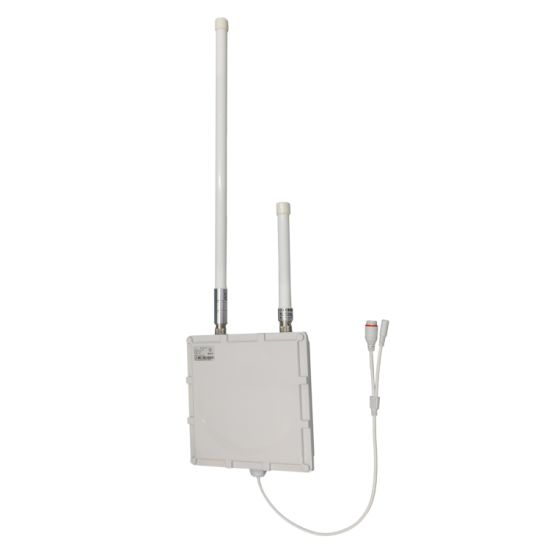
\includegraphics[page=1,width=0.4\paperwidth]{presentation.tex/fig/gateway.jpg}}
  \end{column}
\end{columns}
\end{frame}

\begin{frame}{LoRaWAN}
\framesubtitle{Un protocole MAC ?}

\begin{block}{MAC}
Elle sert d'interface entre la partie logicielle contrôlant la 
liaison d'un nœud (Contrôle de la liaison logique) et la couche 
physique (matérielle). Par conséquent, elle est différente selon 
le type de média physique utilisé (Ethernet, WLAN, …)
\end{block}

\end{frame}

\begin{frame}{LoRaWAN}
\framesubtitle{Aloha}
\begin{block}{}
{
  Quel moyen le plus simple d'interfacer la couche la couche physique ?
}
\end{block}
\begin{columns}
\begin{column}{0.5\textwidth}
\begin{center}
\scalebox{0.7}{
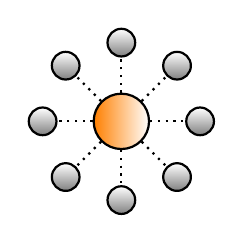
\begin{tikzpicture}[auto, thick]
    \tikzstyle{motes}=[draw,circle,bottom color= gray,
                      top color= white,minimum width=10pt]
    \tikzstyle{gateways}=[draw,circle, left color= orange,minimum width=20pt]
    \foreach \place/\name in {{(0,0)/a}}
        \node[gateways] (\name) at \place {};
    % Place normal peers
    \foreach \pos/\i in {below left of/1, below of/2, left of/3, above left of/4, below right of/5,above of/6, right of/7, above right of/8}
        \node[motes, \pos =a ] (a\i) {};
    \foreach \speer/\peer in {a/a1,a/a2,a/a3,a/a4,a/a5,a/a6,a/a7,a/a8}
        \path[dotted] (\speer) edge (\peer);
\end{tikzpicture}
}
\end{center}
\begin{center}
\scalebox{0.5}{%
\begin{tabular}{r@{ }l r@{ }l}

\begin{tikzpicture}\draw[left color=orange,line width=1pt] circle(1ex);\end{tikzpicture} & Gateway & 
\begin{tikzpicture}\draw[left color=gray,line width=1pt] circle(1ex);\end{tikzpicture} & Mote
\end{tabular}
}
\end{center}
\end{column}
\begin{column}{0.5\textwidth}
\begin{center}
  \scalebox{0.6}{
  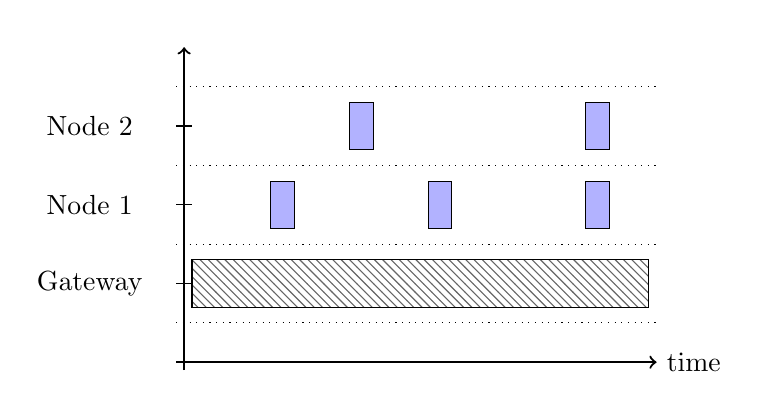
\begin{tikzpicture}[
    ack/.style={draw, rectangle, fill=orange!40, inner sep=0pt, outer sep=0pt},
    tx/.style={draw, rectangle, fill=blue!30,inner sep=0pt, outer sep=0pt},
    relay/.style={draw, rectangle, fill=green!30,inner sep=0pt, outer sep=0pt},
    rx/.style={draw, pattern=north west lines, pattern color=black!60, rectangle, inner sep=0pt, outer sep=0pt},
    arr/.style={help lines,black!70,<->},
    ]
    \draw[->,thick] (-0.1,0)--(6,0) node[right]{time};
    \draw[->,thick] (0,-0.1)--(0,4) node[above]{};

    \draw[dotted] (-0.1,0.5)--(6,0.5);
    \node[] at (-1.2, 1) {Gateway};
    \draw[] (-0.1,1)--(0.1,1);
    \draw[dotted] (-0.1,1.5)--(6,1.5);
    \node[] at (-1.2, 2) {Node 1};
    \draw[] (-0.1,2)--(0.1,2);
    \draw[dotted] (-0.1,2.5)--(6,2.5);
    \node[] at (-1.2, 3) {Node 2};
    \draw[] (-0.1,3)--(0.1,3);
    \draw[dotted] (-0.1,3.5)--(6,3.5);

    % Gateway
    \node () [rx, fit={(0.1,0.7) (5.9,1.3)}] {};
    % Relay
    \node () [tx, fit={(1.1,1.7) (1.4,2.3)}] {};
    \node () [tx, fit={(3.1,1.7) (3.4,2.3)}] {};
    \node () [tx, fit={(5.1,1.7) (5.4,2.3)}] {};
    % Node
    \node () [tx, fit={(2.1,2.7) (2.4,3.3)}] {};
    \node () [tx, fit={(5.1,2.7) (5.4,3.3)}] {};
  \end{tikzpicture}
  }
  % \caption{Collision between nodes}
  \scalebox{0.6}{
  \begin{tabular}{r@{ }l r@{ }l}
  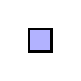
\begin{tikzpicture}\draw[fill=blue!30,line width=1pt] +(-4pt,-4pt) rectangle +(4pt,4pt);\end{tikzpicture} & Transmission 
    & 
\begin{tikzpicture}\draw[pattern=north west lines, pattern color=black!90,line width=1pt] +(-4pt,-4pt) rectangle +(4pt,4pt);\end{tikzpicture} & Reception
  \end{tabular}
  }
\end{center}
\end{column}
\end{columns}

\end{frame}

\begin{frame}{LoRaWAN}
\framesubtitle{Acknowledgement}
\begin{block}{}
{
  Comment s'assurer de la récèption du message ?
}
\end{block}
\begin{columns}
\begin{column}{0.4\textwidth}
\begin{center}
\scalebox{0.7}{
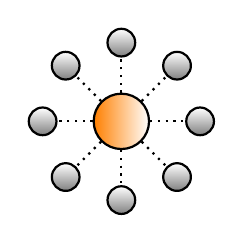
\begin{tikzpicture}[auto, thick]
    \tikzstyle{motes}=[draw,circle,bottom color= gray,
                      top color= white,minimum width=10pt]
    \tikzstyle{gateways}=[draw,circle, left color= orange,minimum width=20pt]
    \foreach \place/\name in {{(0,0)/a}}
        \node[gateways] (\name) at \place {};
    % Place normal peers
    \foreach \pos/\i in {below left of/1, below of/2, left of/3, above left of/4, below right of/5,above of/6, right of/7, above right of/8}
        \node[motes, \pos =a ] (a\i) {};
    \foreach \speer/\peer in {a/a1,a/a2,a/a3,a/a4,a/a5,a/a6,a/a7,a/a8}
        \path[dotted] (\speer) edge (\peer);
\end{tikzpicture}
}
\end{center}
\begin{center}
\scalebox{0.6}{%
\begin{tabular}{r@{ }l r@{ }l}

\begin{tikzpicture}\draw[left color=orange,line width=1pt] circle(1ex);\end{tikzpicture} & Gateway & 
\begin{tikzpicture}\draw[left color=gray,line width=1pt] circle(1ex);\end{tikzpicture} & Mote
\end{tabular}
}
\end{center}
\end{column}
\begin{column}{0.5\textwidth}
\begin{center}
  \scalebox{0.6}{
  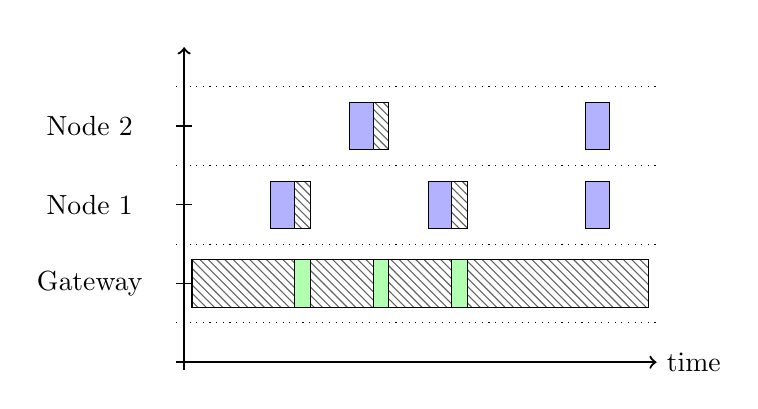
\begin{tikzpicture}[
    ack/.style={draw, rectangle, fill=orange!40, inner sep=0pt, outer sep=0pt},
    tx/.style={draw, rectangle, fill=blue!30,inner sep=0pt, outer sep=0pt},
    relay/.style={draw, rectangle, fill=green!30,inner sep=0pt, outer sep=0pt},
    rx/.style={draw, pattern=north west lines, pattern color=black!60, rectangle, inner sep=0pt, outer sep=0pt},
    arr/.style={help lines,black!70,<->},
    ]
    \draw[->,thick] (-0.1,0)--(6,0) node[right]{time};
    \draw[->,thick] (0,-0.1)--(0,4) node[above]{};

    \draw[dotted] (-0.1,0.5)--(6,0.5);
    \node[] at (-1.2, 1) {Gateway};
    \draw[] (-0.1,1)--(0.1,1);
    \draw[dotted] (-0.1,1.5)--(6,1.5);
    \node[] at (-1.2, 2) {Node 1};
    \draw[] (-0.1,2)--(0.1,2);
    \draw[dotted] (-0.1,2.5)--(6,2.5);
    \node[] at (-1.2, 3) {Node 2};
    \draw[] (-0.1,3)--(0.1,3);
    \draw[dotted] (-0.1,3.5)--(6,3.5);

    % Gateway
    \node () [rx, fit={(0.1,0.7) (5.9,1.3)}] {};
    \node () [relay, fit={(1.4,0.7) (1.6,1.3)}] {};
    \node () [relay, fit={(3.4,0.7) (3.6,1.3)}] {};
    \node () [relay, fit={(2.4,0.7) (2.6,1.3)}] {};
    % Relay
    \node () [tx, fit={(1.1,1.7) (1.4,2.3)}] {};
    \node () [rx, fit={(1.4,1.7) (1.6,2.3)}] {};
    \node () [tx, fit={(3.1,1.7) (3.4,2.3)}] {};
    \node () [rx, fit={(3.4,1.7) (3.6,2.3)}] {};
    \node () [tx, fit={(5.1,1.7) (5.4,2.3)}] {};
    % Node
    \node () [tx, fit={(2.1,2.7) (2.4,3.3)}] {};
    \node () [rx, fit={(2.4,2.7) (2.6,3.3)}] {};
    \node () [tx, fit={(5.1,2.7) (5.4,3.3)}] {};
  \end{tikzpicture}
  }
  % \caption{Collision between nodes}
  \scalebox{0.6}{
  \begin{tabular}{r@{ }l r@{ }l}
  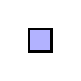
\begin{tikzpicture}\draw[fill=blue!30,line width=1pt] +(-4pt,-4pt) rectangle +(4pt,4pt);\end{tikzpicture} & Transmission 
    & 
\begin{tikzpicture}\draw[pattern=north west lines, pattern color=black!90,line width=1pt] +(-4pt,-4pt) rectangle +(4pt,4pt);\end{tikzpicture} & Reception
  \end{tabular}
  }
\end{center}
\end{column}
\end{columns}

\end{frame}

\begin{frame}{LoRaWAN}
\framesubtitle{Retransmission}
\begin{center}
\scalebox{0.6}{
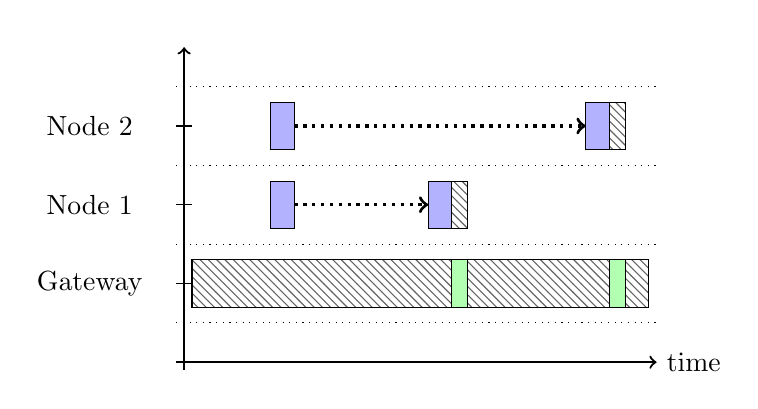
\begin{tikzpicture}[
  ack/.style={draw, rectangle, fill=orange!40, inner sep=0pt, outer sep=0pt},
  tx/.style={draw, rectangle, fill=blue!30,inner sep=0pt, outer sep=0pt},
  relay/.style={draw, rectangle, fill=green!30,inner sep=0pt, outer sep=0pt},
  rx/.style={draw, pattern=north west lines, pattern color=black!60, rectangle, inner sep=0pt, outer sep=0pt},
  arr/.style={help lines,black!70,<->},
  ]
  \draw[->,thick] (-0.1,0)--(6,0) node[right]{time};
  \draw[->,thick] (0,-0.1)--(0,4) node[above]{};

  \draw[dotted] (-0.1,0.5)--(6,0.5);
  \node[] at (-1.2, 1) {Gateway};
  \draw[] (-0.1,1)--(0.1,1);
  \draw[dotted] (-0.1,1.5)--(6,1.5);
  \node[] at (-1.2, 2) {Node 1};
  \draw[] (-0.1,2)--(0.1,2);
  \draw[dotted] (-0.1,2.5)--(6,2.5);
  \node[] at (-1.2, 3) {Node 2};
  \draw[] (-0.1,3)--(0.1,3);
  \draw[dotted] (-0.1,3.5)--(6,3.5);

  \draw[->,very thick,dotted] (1.4,2)--(3.1,2);
  \draw[->,very thick,dotted] (1.4,3)--(5.1,3);

  % Gateway
  \node () [rx, fit={(0.1,0.7) (5.9,1.3)}] {};
  \node () [relay, fit={(3.4,0.7) (3.6,1.3)}] {};
  \node () [relay, fit={(5.4,0.7) (5.6,1.3)}] {};
  % Node 1
  \node () [tx, fit={(1.1,1.7) (1.4,2.3)}] {};
  \node () [tx, fit={(3.1,1.7) (3.4,2.3)}] {};
  \node () [rx, fit={(3.4,1.7) (3.6,2.3)}] {};
  % Node 2
  \node () [tx, fit={(1.1,2.7) (1.4,3.3)}] {};
  \node () [tx, fit={(5.1,2.7) (5.4,3.3)}] {};
  \node () [rx, fit={(5.4,2.7) (5.6,3.3)}] {};
\end{tikzpicture}
}
\end{center}
\begin{center}
\scalebox{0.6}{
\begin{tabular}{r@{ }l r@{ }l}
  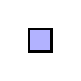
\begin{tikzpicture}\draw[fill=blue!30,line width=1pt] +(-4pt,-4pt) rectangle +(4pt,4pt);\end{tikzpicture} & Transmission 
    & 
\begin{tikzpicture}\draw[pattern=north west lines, pattern color=black!90,line width=1pt] +(-4pt,-4pt) rectangle +(4pt,4pt);\end{tikzpicture} & Reception
\end{tabular}
}
\end{center}

\end{frame}

\begin{frame}{LoRaWAN}
\framesubtitle{Multiplexing}
\begin{block}{}
{
  Comment éviter les colisions ?
}
\end{block}
\begin{center}
\scalebox{0.6}{
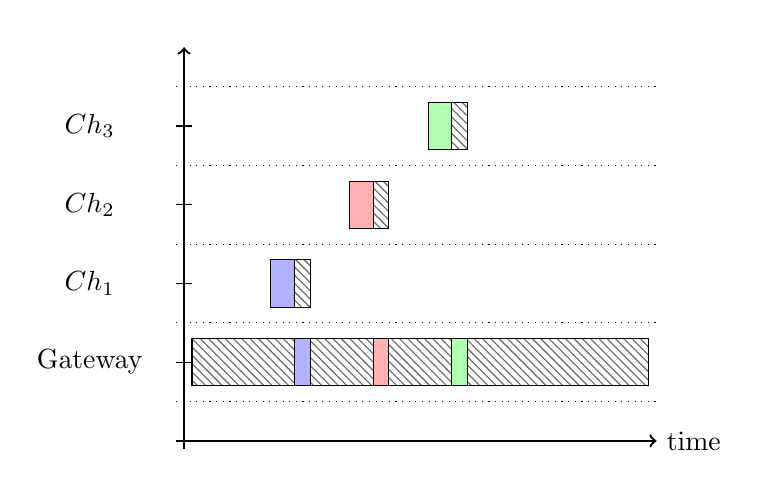
\begin{tikzpicture}[
  ack/.style={draw, rectangle, fill=orange!40, inner sep=0pt, outer sep=0pt},
  tx/.style={draw, rectangle, inner sep=0pt, outer sep=0pt},
  ch1/.style={fill=blue!30},
  ch2/.style={fill=red!30},
  ch3/.style={fill=green!30},
  rx/.style={draw, pattern=north west lines, pattern color=black!60, rectangle, inner sep=0pt, outer sep=0pt},
  arr/.style={help lines,black!70,<->},
  ]
  \draw[->,thick] (-0.1,0)--(6,0) node[right]{time};
  \draw[->,thick] (0,-0.1)--(0,5) node[above]{};

  \draw[dotted] (-0.1,0.5)--(6,0.5);
  \node[] at (-1.2, 1) {Gateway};
  \draw[] (-0.1,1)--(0.1,1);
  \draw[dotted] (-0.1,1.5)--(6,1.5);
  \node[] at (-1.2, 2) {$Ch_{1}$};
  \draw[] (-0.1,2)--(0.1,2);
  \draw[dotted] (-0.1,2.5)--(6,2.5);
  \node[] at (-1.2, 3) {$Ch_{2}$};
  \draw[] (-0.1,3)--(0.1,3);
  \draw[dotted] (-0.1,3.5)--(6,3.5);
  \node[] at (-1.2, 4) {$Ch_{3}$};
  \draw[] (-0.1,4)--(0.1,4);
  \draw[dotted] (-0.1,4.5)--(6,4.5);

  % Gateway
  \node () [rx, fit={(0.1,0.7) (5.9,1.3)}] {};
  \node () [tx, ch1, fit={(1.4,0.7) (1.6,1.3)}] {};
  \node () [tx, ch2, fit={(2.4,0.7) (2.6,1.3)}] {};
  \node () [tx, ch3, fit={(3.4,0.7) (3.6,1.3)}] {};
  % Ch 1
  \node () [tx, ch1, fit={(1.1,1.7) (1.4,2.3)}] {};
  \node () [rx, fit={(1.4,1.7) (1.6,2.3)}] {};
  % Ch 2
  \node () [tx, ch2, fit={(2.1,2.7) (2.4,3.3)}] {};
  \node () [rx, fit={(2.4,2.7) (2.6,3.3)}] {};
  % Ch 3
  \node () [tx, ch3, fit={(3.1,3.7) (3.4,4.3)}] {};
  \node () [rx, fit={(3.4,3.7) (3.6,4.3)}] {};
\end{tikzpicture}
}
\end{center}
\begin{center}
\scalebox{0.6}{
\begin{tabular}{r@{ }l r@{ }l}
  
\begin{tikzpicture}\draw[pattern=north west lines, pattern color=black!90,line width=1pt] +(-4pt,-4pt) rectangle +(4pt,4pt);\end{tikzpicture} & Reception
    & 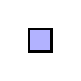
\begin{tikzpicture}\draw[fill=blue!30,line width=1pt] +(-4pt,-4pt) rectangle +(4pt,4pt);\end{tikzpicture} & Channel 1 \\
  
\begin{tikzpicture}\draw[fill=red!30,line width=1pt] +(-4pt,-4pt) rectangle +(4pt,4pt);\end{tikzpicture} & Channel 2
    & 
\begin{tikzpicture}\draw[fill=green!30,line width=1pt] +(-4pt,-4pt) rectangle +(4pt,4pt);\end{tikzpicture} & Channel 3
\end{tabular}
}
\end{center}

\end{frame}

\begin{frame}{LoRaWAN}
\framesubtitle{Adaptive Data Rate}
\begin{block}{}
{
  Comment étendre la portée ?
}
\end{block}
\begin{columns}
\begin{column}{0.5\textwidth}
\begin{center}
\scalebox{0.8}{
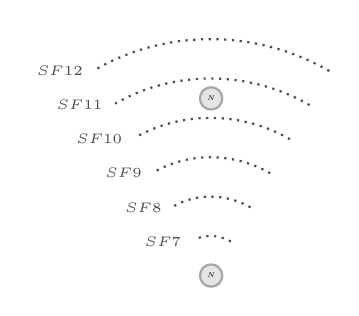
\begin{tikzpicture}[
    state/.style={circle, thick,draw=gray!70,fill=gray!20,text=black,scale=0.5},
]
\tikzset{
  pics/carc/.style args={#1:#2:#3:#4}{
    code={
      \draw[pic actions] (#1:#3) arc(#1:#2:#3) node[at end,left, black!70] {\tiny #4};
    }
  }
}
\begin{scope}[shorten >=1pt,auto,node distance=4.5cm]
  \node[state]         (A) [] {\tiny $N$};
  \node[state]         (B) [below of=A]       {\tiny $N$};
  \draw[black!70, dotted, thick] (B) pic{carc=60:120:0.5cm:$SF7$}
    pic{carc=60:120:1cm:$SF8$} pic{carc=60:120:1.5cm:$SF9$}
    pic{carc=60:120:2cm:$SF10$} pic{carc=60:120:2.5cm:$SF11$}
    pic{carc=60:120:3cm:$SF12$};
\end{scope}
\end{tikzpicture}
}
\end{center}
\end{column}
\begin{column}{0.5\textwidth}
\begin{center}
\scalebox{0.6}{
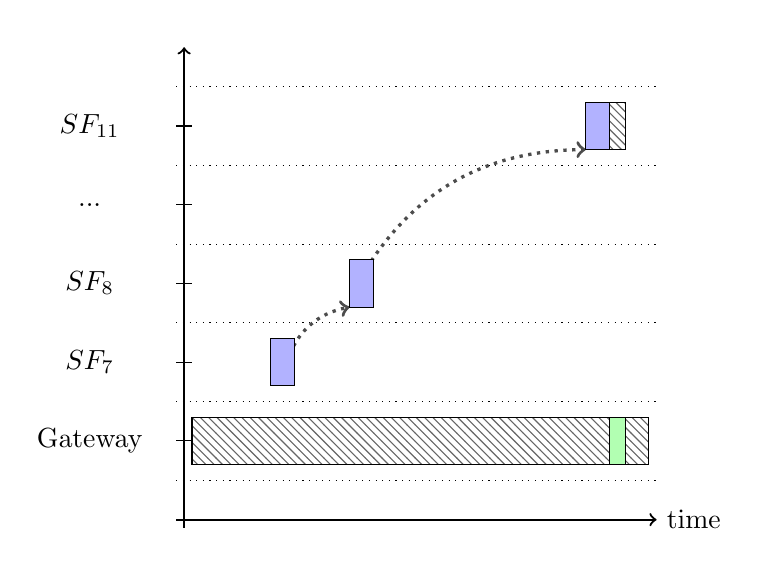
\begin{tikzpicture}[
  ack/.style={draw, rectangle, fill=orange!40, inner sep=0pt, outer sep=0pt},
  tx/.style={draw, rectangle, fill=blue!30,inner sep=0pt, outer sep=0pt},
  relay/.style={draw, rectangle, fill=green!30,inner sep=0pt, outer sep=0pt},
  rx/.style={draw, pattern=north west lines, pattern color=black!60, rectangle, inner sep=0pt, outer sep=0pt},
  arr/.style={help lines,black!70,<->},
  ]
  \draw[->,thick] (-0.1,0)--(6,0) node[right]{time};
  \draw[->,thick] (0,-0.1)--(0,6) node[above]{};

  \draw[dotted] (-0.1,0.5)--(6,0.5);
  \node[] at (-1.2, 1) {Gateway};
  \draw[] (-0.1,1)--(0.1,1);
  \draw[dotted] (-0.1,1.5)--(6,1.5);
  \node[] at (-1.2, 2) {$SF_{7}$};
  \draw[] (-0.1,2)--(0.1,2);
  \draw[dotted] (-0.1,2.5)--(6,2.5);
  \node[] at (-1.2, 3) {$SF_{8}$};
  \draw[] (-0.1,3)--(0.1,3);
  \draw[dotted] (-0.1,3.5)--(6,3.5);
  \node[] at (-1.2, 4) {$...$};
  \draw[] (-0.1,4)--(0.1,4);
  \draw[dotted] (-0.1,4.5)--(6,4.5);
  \node[] at (-1.2, 5) {$SF_{11}$};
  \draw[] (-0.1,5)--(0.1,5);
  \draw[dotted] (-0.1,5.5)--(6,5.5);

  \path (1.3,2) edge[->,dotted,very thick,bend left,black!70] (2.1,2.7);
  \path (2.2,3) edge[->,dotted,very thick,bend left,black!70] (5.1,4.7);

  % Gateway
  \node () [rx, fit={(0.1,0.7) (5.9,1.3)}] {};
  \node () [relay, fit={(5.4,0.7) (5.6,1.3)}] {};
  % SF7
  \node () [tx, fit={(1.1,1.7) (1.4,2.3)}] {};
  % SF8
  \node () [tx, fit={(2.1,2.7) (2.4,3.3)}] {};
  % ...
  % SF11
  \node () [tx, fit={(5.1,4.7) (5.4,5.3)}] {};
  \node () [rx, fit={(5.4,4.7) (5.6,5.3)}] {};
\end{tikzpicture}
}
% \caption{Collision between nodes}
\scalebox{0.6}{
\begin{tabular}{r@{ }l r@{ }l}
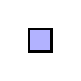
\begin{tikzpicture}\draw[fill=blue!30,line width=1pt] +(-4pt,-4pt) rectangle +(4pt,4pt);\end{tikzpicture} & Transmission 
  & 
\begin{tikzpicture}\draw[pattern=north west lines, pattern color=black!90,line width=1pt] +(-4pt,-4pt) rectangle +(4pt,4pt);\end{tikzpicture} & Reception
\end{tabular}
}
\end{center}
\end{column}
\end{columns}

\end{frame}

\begin{frame}{LoRaWAN}
\framesubtitle{Pourquoi ce succès ?}
\begin{itemize}
  \item LoRaWAN est open source contrairement à ses concurrents
  \item Possible de créer son réseau privé  
  \item Possible de créer son propre protocol utilisant LoRa PHY
  \item The Things Network
  \begin{itemize}
    \item Réseau LoRaWAN crowdfunder
    \item Offrir sa gateway à d'autres utilisateurs
  \end{itemize}
\end{itemize}
\end{frame}

\begin{frame}{LoRaWAN}
\framesubtitle{Aller plus loin}
\begin{itemize}
  \item Limitation pour le downlink
\end{itemize}
\end{frame}


\section{RIOT}

\subsection{Introduction}

\begin{frame}{RIOT}
\framesubtitle{Introduction}
\begin{columns}
\begin{column}{0.5\textwidth}
 \begin{itemize}
  \item Un OS pour l'IoT
  \begin{itemize}
    \item CAN
    \item BLE (NimBLE)
    \item LoRaWAN
    \item SigFox
    \item 6LoWPAN, Thread
  \end{itemize}
  \item Tickless scheduler
  \begin{itemize}
    \item Basse consommation
  \end{itemize}
  \item Temps reel
  \item API pour les drivers
  \item build, flash et console facile
  \begin{itemize}
    \item \lstinline{make flash term}
  \end{itemize}
\end{itemize}
\end{column}
\begin{column}{0.5\textwidth}
\makebox[\linewidth]{
\includegraphics[width=\textwidth]{presentation.tex/fig/riot.png}}
\end{column}
\end{columns}
\end{frame}

\begin{frame}{RIOT}
\framesubtitle{Introduction}
\begin{center}
\scalebox{0.45}{%
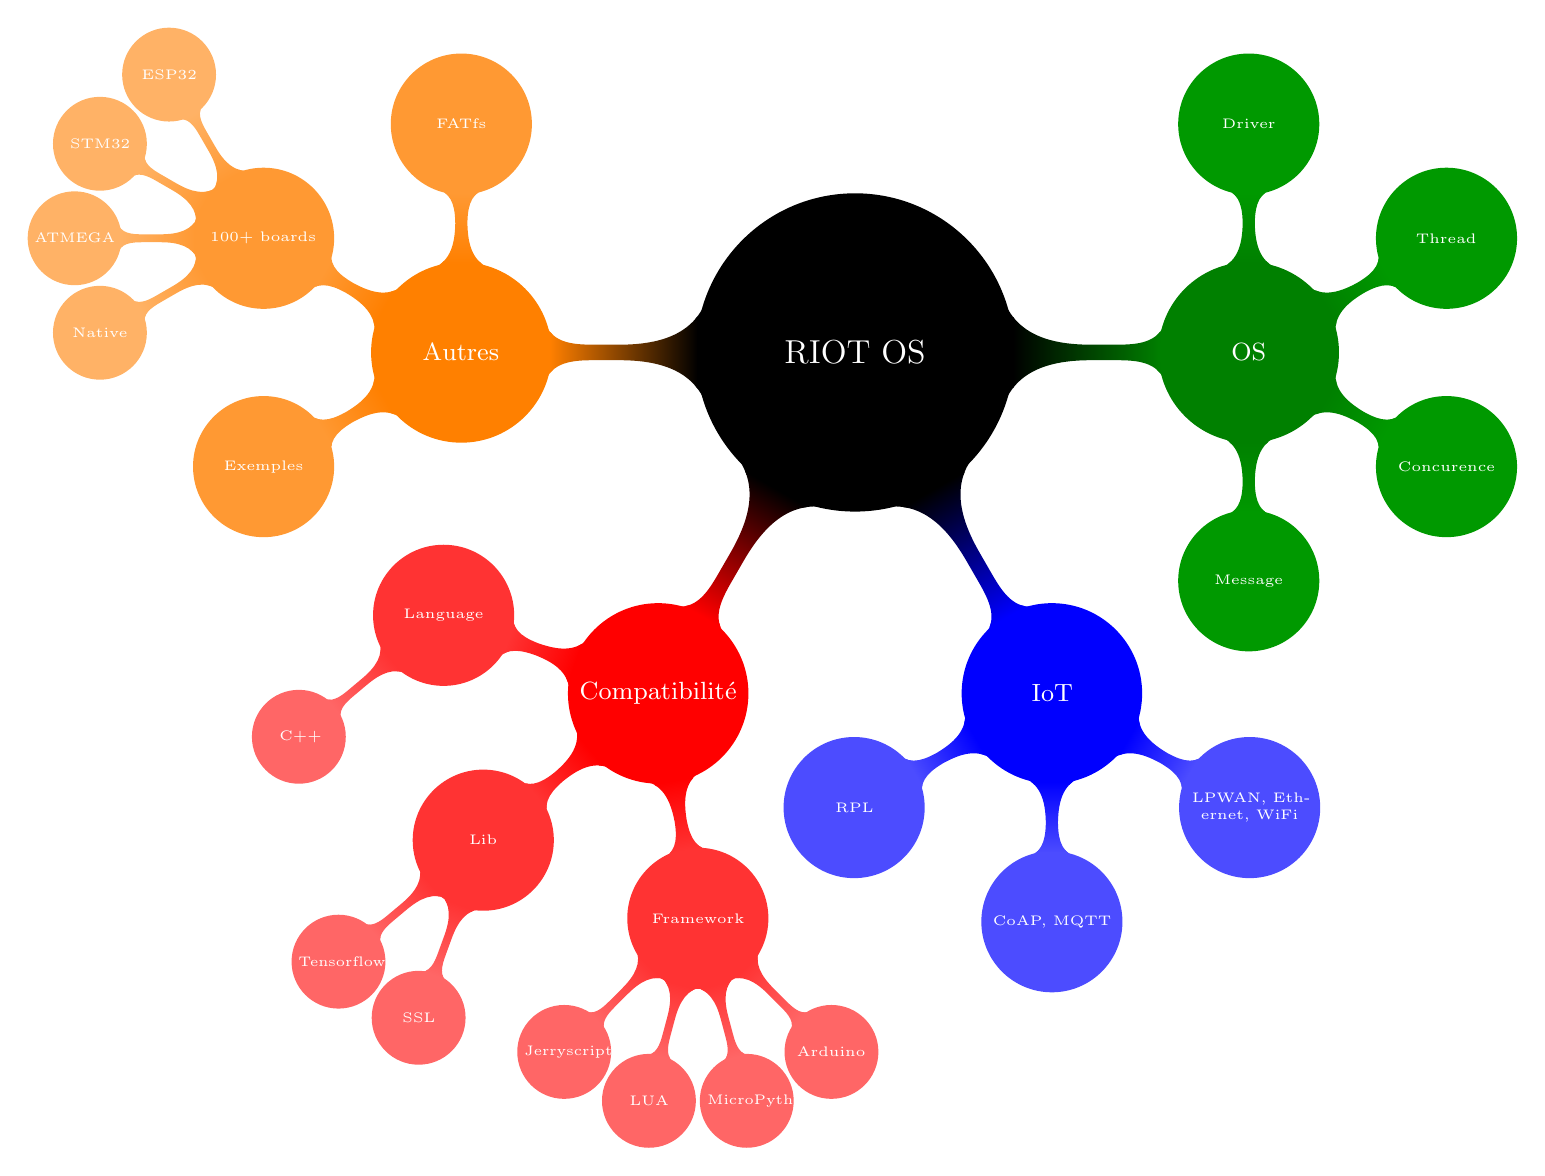
\begin{tikzpicture}
\path[mindmap,concept color=black,text=white]
  node[concept] {RIOT OS}
  [clockwise from=0]
  child[concept color=green!50!black] {
    node[concept] {OS}
    [clockwise from=90]
    child[concept color=green!60!black] { node[concept] {Driver} }
    child[concept color=green!60!black] { node[concept] {Thread} }
    child[concept color=green!60!black] { node[concept] {Concurence} }
    child[concept color=green!60!black] { node[concept] {Message} }
  }  
  child[concept color=blue] {
    node[concept] {IoT}
    [clockwise from=-30]
    child[concept color=blue!70] { node[concept] {LPWAN, Ethernet, WiFi} }
    child[concept color=blue!70] { node[concept] {CoAP, MQTT} }
    child[concept color=blue!70] { node[concept] {RPL} }
  }
  child[concept color=red] { 
    node[concept] {Compatibilité} 
    [clockwise from=-80]
    child[concept color=red!80]  { 
      node[concept] {Framework} 
      [clockwise from=-45]
      child[concept color=red!60] { node[concept] {Arduino} }
      child[concept color=red!60] { node[concept] {MicroPython} }
      child[concept color=red!60] { node[concept] {LUA} }
      child[concept color=red!60] { node[concept] {Jerryscript} }
    }
    child[concept color=red!80]  { 
      node[concept] {Lib} 
      [counterclockwise from=-140]
      child[concept color=red!60] { node[concept] {Tensorflow} }
      child[concept color=red!60] { node[concept] {SSL} }
    }
    child[concept color=red!80]  { 
      node[concept] {Language} 
      [counterclockwise from=-140]
      child[concept color=red!60] { node[concept] {C++} }
    }
  }
  child[concept color=orange] { 
    node[concept] {Autres} 
    [counterclockwise from=90]
    child[concept color=orange!80] { node[concept] {FATfs} }
    child[concept color=orange!80] { 
      node[concept] {100+ boards} 
      [counterclockwise from=120]
      child[concept color=orange!60] { node[concept] {ESP32} }
      child[concept color=orange!60] { node[concept] {STM32} }
      child[concept color=orange!60] { node[concept] {ATMEGA} }
      child[concept color=orange!60] { node[concept] {Native} }
    }
    child[concept color=orange!80] { node[concept] {Exemples} }
  };
\end{tikzpicture}
}
\end{center}

\end{frame}

\begin{frame}{RIOT}
\framesubtitle{Concurrence}
\begin{columns}
\begin{column}{0.6\textwidth}
 \begin{itemize}
  \item Une approche 'from scratch'
  \begin{itemize}
    \item Pas de dependance constructeur
    \item Driver maison
  \end{itemize}
  \item Communauté accessible
  \item Beaucoups de drivers
  \item Beaucoups de plateformes
  \begin{itemize}
    \item Support pour le low-end
    \item Support CPU 8, 16 bits
  \end{itemize}
\end{itemize}
\end{column}
\begin{column}{0.4\textwidth}
\begin{center}
  
\includegraphics[width=0.9\textwidth]{presentation.tex/fig/armmbed.png}
  
\includegraphics[width=0.8\textwidth]{presentation.tex/fig/zephyr.png}
\end{center}
\end{column}
\end{columns}
\end{frame}

\subsection{Utilisation}

\begin{frame}[t]
  \frametitle{RIOT}
  \framesubtitle{Utilisation}
\end{frame}



\begin{frame}{Backup}
\framesubtitle{LoRa vs Sigfox}
\begin{itemize}
  \item MAC propriétaire
  \item Abonnement, réseaux privés par les opérateurs téléphoniques
  \item 140 messages de 12 bytes uplink
  \item 4 messages en downlink
\end{itemize}
\end{frame}

\begin{frame}{Backup}
\framesubtitle{LoRa vs NB-IoT}
\begin{itemize}
  \item Se base sur l'infrastructure LTE
  \item Abonnement, réseaux privés par les opérateurs téléphoniques
\end{itemize}
\end{frame}



\end{document}

